\section{Annexes}

\renewcommand{\figurename}{Annexe}
\captionsetup{list=no}

\setcounter{figure}{0}

\appendices{Résultats du filtre de Canny sur des couleurs de peau différentes}
\begin{figure}[H]
  \center
  \begin{tabular}{|c|c|}
    \hline
    Image originale & Image après filtre de Canny\\
    \hline
    
\includegraphics{image/original.png} & 
\includegraphics{image/canny_final.png}\\
    \hline
    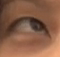
\includegraphics{image/original_asiatique.png} & 
\includegraphics{image/cannyAsiatique.png}\\
    \hline
    
\includegraphics{image/original_black.png} & 
\includegraphics{image/cannyBlack.png}\\
    \hline
  \end{tabular}
  \caption{Résultats du filtre de Canny sur des personnes de couleur de peau différentes}
\end{figure}

\appendices{Comparatif des histogrammmes du canal Cb, selon les traitement}
\begin{figure}[H]
  \center
  \begin{tabular}{|c|c|c|c|}
    \hline
      Image RGB & Canal Cb de YCbCr & Canal Cb égalisé & Canal Cb normalisé \\
    \hline
      \shortstack{
\includegraphics[width=3.3cm]{image/008/rgb_source.png}           \\ 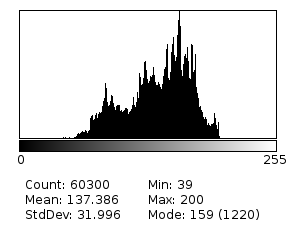
\includegraphics[width=3.3cm]{image/008/rgb_source_hist.png}} &
      \shortstack{
\includegraphics[width=3.3cm]{image/008/ycbcr_ch1.png}            \\ 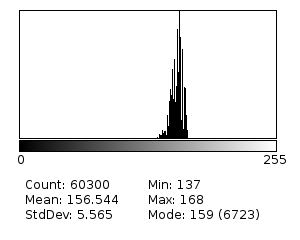
\includegraphics[width=3.3cm]{image/008/ycbcr_ch1_hist.png}} &
      \shortstack{
\includegraphics[width=3.3cm]{image/008/ycbcr_ch1_equalized.png}  \\ 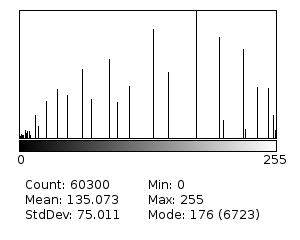
\includegraphics[width=3.3cm]{image/008/ycbcr_ch1_equalized_hist.png}} &
      \shortstack{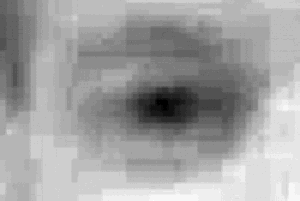
\includegraphics[width=3.3cm]{image/008/ycbcr_ch1_normalized.png} \\ 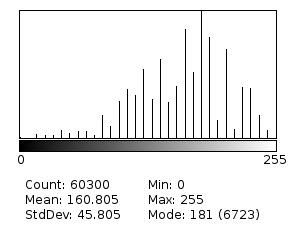
\includegraphics[width=3.3cm]{image/008/ycbcr_ch1_normalized_hist.png}}\\
    \hline
      \shortstack{
\includegraphics[width=3.3cm]{image/017/rgb_source.png}           \\ 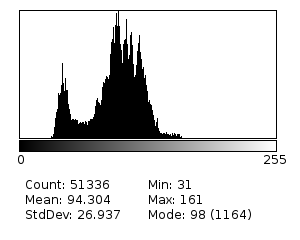
\includegraphics[width=3.3cm]{image/017/rgb_source_hist.png}} &
      \shortstack{
\includegraphics[width=3.3cm]{image/017/ycbcr_ch1.png}            \\ 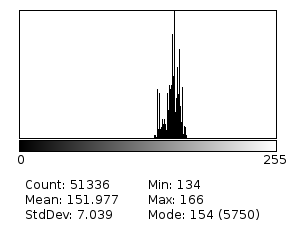
\includegraphics[width=3.3cm]{image/017/ycbcr_ch1_hist.png}} &
      \shortstack{
\includegraphics[width=3.3cm]{image/017/ycbcr_ch1_equalized.png}  \\ 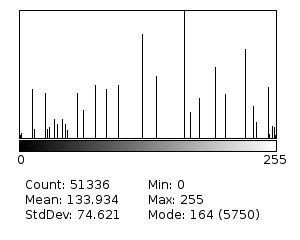
\includegraphics[width=3.3cm]{image/017/ycbcr_ch1_equalized_hist.png}} &
      \shortstack{
\includegraphics[width=3.3cm]{image/017/ycbcr_ch1_normalized.png} \\ 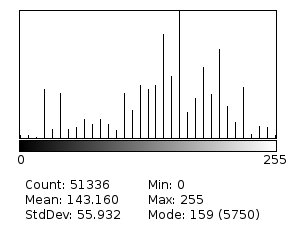
\includegraphics[width=3.3cm]{image/017/ycbcr_ch1_normalized_hist.png}}\\
    \hline
    %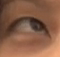
\includegraphics{image/original_asiatique.png} & 
\includegraphics{image/cannyAsiatique.png}\\
    %\hline
    %
\includegraphics{image/original_black.png} & 
\includegraphics{image/cannyBlack.png}\\
    %\hline
  \end{tabular}
  \caption{Comparatif des histogrammmes du canal Cb, selon les traitement}
\end{figure}

\newpage